1. $\cfrac{(x^2-4x+3)(x-3)(x^2+2x+3)}{(x^2+x-20)(x+2)^2}\geqslant0 \Leftrightarrow \cfrac{(x-1)(x-3)^2((x+1)^2+2)}{(x-4)(x+5)(x+2)^2}\geqslant0.$ Применив метод интервалов, найдём ответ: $x\in(-5;-2)\cup(-2;1]\cup\{3\}\cup(4;+\infty).$
\begin{figure}[ht!]
\center{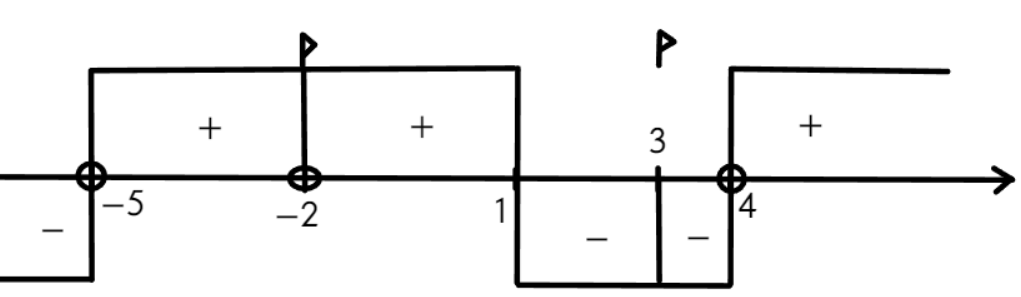
\includegraphics[scale=0.35]{ner9-1.png}}
\end{figure}\\
